% set counter to n-1:
\setcounter{chapter}{1}

\chapter{Related Work}

Sample references are~\cite{Zwicker04Perspective} and~\cite{Altman89QuaternionScandal}.



\section{Robustness Overview} \label{Robustness Overview}
Robustness is a desirable property of robotic systems as it allows them to navigate uncertain environments without system failure. At the same time, finding concrete measures for quantifying robustness is difficult, especially when striving for a generality, as often definitions are either vague or overly specific.
This section provides an overview of differenct interpretations of the concept. 



\subsection{The Robustness Principle} \label{The Robustness Principle}
%\subsubsection{Sub-Sub-Category (if necessary)}
The Transmission Control Protocol from 1981 ~\cite{trm}, which contains guidelines for host-to-host communication via networks, states: “Be conservative in what you do, be liberal in what you accept from others”. The idea being that sent out data should be as concise as possible, while on the receiving side deviations from the standard should be accounted for. Translated to our problem, a robot behaves robustly when it successfully executes concisely given commands even in the presence of unexpected disturbances. To achieve this a margin of error should always be accounted for to bridge the gap between theory and practice.




\subsection{Robustness against Failure} \label{Robustness against Failure}
N. Hazon et al.\ \cite{covrob} have improved upon multi-agent algorithms for coverage  to account for failure of agents. Here robustness was quantified by proving that the presented algorithms would always succeed, as long as at least one functioning agent remains. On a similar note, M. Hofbaur et al.\ \cite{sysrob} have worked on making mobile robots robust against failure, however here robustness was defined with respect to unexpected internal changes, for example the failure of an actuator. The issue with these failures is that the robot is usually unaware and continues to try to use the broken component, resulting in the failure of the entire robot. By actively monitoring the system and changing the internal model, the robot is often able to overcome its impairment. In both cases, robustness is merely a binary measure and its value can be quantified quite decisively. In contrast, the problem at hand seeks a measure that can be evaluated continuously, especially as the robustness is to be optimized and to be compared between different designs. 
 

\subsection{Robust Optimization} \label{Robust Optimization}
Robust optimization is an extension to ordinary optimization problems, in which uncertainty sets are introduced as additional parameters, as described and summarized by \cite{optrob}. The argument goes that if a solution is feasible not for only one parameter but covers a set of uncertainties, it will in turn be generally robust against them. While optimally the solution would be robust against any arbitrary uncertainty, covering a larger amount of cases usually also results in the deterioration of the solution for any particular case. The optimization algorithm is applied to find a balance within this trade-off. While the choice of defining the uncertainties results in different “strengths” of robustness,  there exists no method for measuring the resulting robustness of the solution, meaning that it cannot be assessed independently of the optimization problem. This makes it impossible to compare different systems as optimizing over the same set of uncertainties in different systems in no way guarantees that their behaviour in any specific case will be comparable.


\subsection{Residual Force Polytopes} \label{Residual Force Polytopes}
Residual force polytopes have been used by \cite{respoly} for trajectory optimization on the ANYmal quadruped platform. The approach here is to represent all largest possible outside forces that the system can compensate as a polytope, i.e.\ a high (usually 3) dimensional volume. Here the vector from the actuator to any point on the surface represents the critical force in that direction. The largest sphere that can be placed within a polytope represents the worst case scenario for that actuator. The radius of this sphere can be used as a concrete measure for robustness which encompasses all possible disturbances. Given a rough trajectory, Ferrolho et al.\ \cite{anytraj} were able to perform an optimization with this measure, maximizing the sum of all of the inscribed spheres for a maximally robust position at every point along the trajectory. 
On a first look this seems promising, however there might be a multitude of physical constellations where the end effector resides at the same position, as shown in Figure~\ref{fig:resforce}. Each constellation has a different polytope and therefore a different robustness measure, a problem which becomes worse for systems with high degrees of freedom. This dependence on the specific state renders this measure unfeasible for our problem.
\begin{figure}[ht]
    \centering
    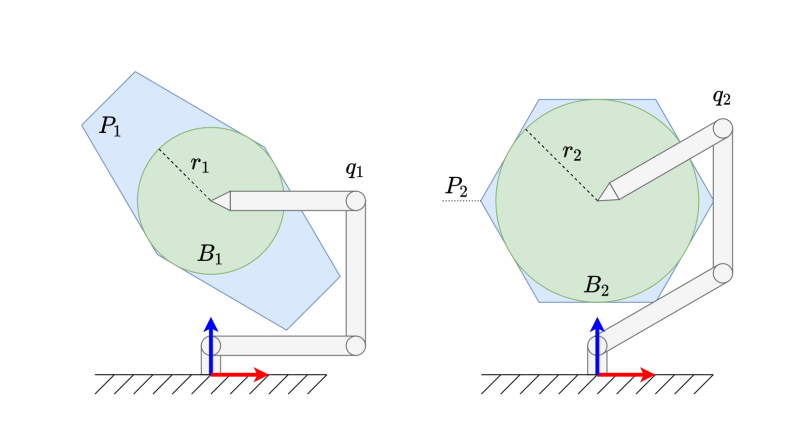
\includegraphics[width=\linewidth]{figures/resdidual_force_polytope}
    \caption[Residual Force Polytopes]{Comparison of two residual force polytopes, with identical endeffector position. The blue area represents the maximal forces the system can compensate with the green circle being the worst case scenario. Note that the shapes change with respect to the configuration of the arm.\cite{respoly}}
    \label{fig:resforce}
\end{figure}


\section{Global Robustness in Nonlinear Dynamic Systems} \label{Global Robustness}
From this it should be evident that the way robustness is defined and quantified strongly depends on the particular application.
For the goal of optimization of dynamical systems with respect to robustness, an unanbiguous quantification is required. As real world systems are compliant and experience impacts, linear system theory is not applicable. There exist however some approaches for dealing with nonlinear dynamical systems, laid out in the following. 

\iffalse
From this it should be evident that the way robustness is defined and quantified strongly depends on the problem it is applied to. The hurdle in finding a measure for the problem at hand is that neither the system nor the applied disturbances are predefined as to preserve generality. Statemen

Analyzing the underlying nonlinear differential equations promises a possibility of making
%To find a suitable solution, it is a good idea to formalize the question to a degree. The mathematical representation of mechanical systems is usually given in the form of differential equations $\dot{\textbf{x}} =F(\textbf{x})$, describing the relationship between the states of a system and their change with respect to time. 
Nonlinearities caused by compliance as well as impacts typically occurring in legged locomotion exclude methods applicable to linear systems of equations. 
What remains are nonlinear systems of differential equations which are to be analyzed and ultimately quantified with respect to robustness. 

\subsection{Phase Space Representation of Dynamic Systems} \label{Phase Space}
A popular method of visualizing dynamic systems are phase space diagrams, which encompass all possible states of a system. For mechanical systems these states are usually the generalized coordinates and their temporal derivatives, where the dimension of the space scales with the degrees of freedom. Solving the differential equations repeatedly, taking various states as the initial conditions, reveals the global behaviour in the form of trajectories within the phase space. An two dimensional example of this can be seen in Figure~\ref{fig:Limitcycle}.

While the trajectories go on indefinitely, most quickly go to infinity or end up in a cyclic pattern. The latter are called attractors, which are of large interest in the discussion of nonlinear dynamic systems. They represent a set of states which the trajectories will not leave once they encounter them. This might represent the repeating motion of a robotic foot at the end of a leg. An important insight here is that around any attractor there exists a set of states who's trajectories will always converge towards the attractor. This set is called the Basin of Attraction (BoA), however it should be noted that the terms “Domain of Attraction”, “Region of Attraction” as well as “Basin Attraction” are used synonymously in literature.
\begin{figure}[ht]
    %\resizebox{.9\linewidth}{!}{\input{plot.tex}}
    \centering
    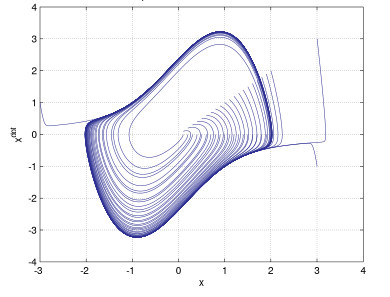
\includegraphics[width=.5\linewidth]{figures/Limitcycle}
    \caption[Phase Space Diagram of a Van der Pol Oscillator]{Phase Space Diagram of a Van der Pol Oscillator. The attractor is indicated by the thick line and the trajectories by thin lines, all converging towards the attractor. \cite{phase}}
    %\scalebox{0.25}{0.25}
    \label{fig:Limitcycle}
\end{figure}
\fi
\subsection{Robustness Measures via the Basin of Attraction} \label{Basin of Attraction}

Given a system which can instantaneously be described by a state, the space spanned by all possible states promises a general approach of analysis. This state space, or phase space (see section \ref{dynamicstheory}), can be partitioned into different regions based on the evolution of states through time. These state trajectories may converge toward a set of states, called the attractor, from a larger surrounding set, called the Basin of Attraction (BoA). Convergence to the attractor is guaranteed for state trajectories starting within the BoA. Disturbances applied to the system may be interpreted as instantaneous state changes, which may move a trajectory outside the BoA, fundamentally changing the future evolution of the system. Attractors may be chosen to represent a desired system behaviour, implying system failure if a disturbance moves the state outside the BoA. The size of the set of states the BoA contains can be used as a robustness measure as a larger BoA implies larger robustness against general disturbances. 
\iffalse
Given that all trajectories starting in the BoA will also always stay within it, a robustness formulation can be derived by taking the effect of disturbances into account. Disturbances generally result in a state changes, which in the context of the phase space corresponds to a jump onto a different trajectory. As long as the new state lies within the BoA, the trajectory will return back to the stable solution and the robot will recover. However if the disturbance is too large, the system will land on a diverging trajectory outside the BoA, quickly leading to failure of the system. To increase robustness, we want to decrease the likelihood of a disturbance moving the system state outside of the basin. Having no control over the types of disturbances that our robot leg might encounter, the geometry of the basin itself needs to be changed. A larger basin will make it more likely that the new trajectory will stay within it, given a random disturbance. The geometry of the BoA is therefore a representation of the system's robustness. To obtain a quantified measure of the robustness, one simple approach is to take the high dimensional volume of the basin.
\fi
Rummel et al.\ \cite{walkbasin} have applied this robustness formulation to identify stable walking gaits in a two degree of freedom spring-mass walker model. In this low dimensional case the size takes shape of the area of the BoA, which was always bounded for the system analyzed. Problematically, these basins may take many complicated forms, including fractals and regions that stretch to infinity. Sprott et al.\ \cite{classify} have come up with a method to sorting the BoA into classes, listed in Table~\ref{t:class} and shown in part in Figure~\ref{fig:classes}. They achieved this by finding a power law describing the probability of a state laying within the basin, depending on it's distance from the attractor. 

\begin{table}[ht]
\centering
\caption[Classes of Basins]{Classes of Basins. \cite{classify}}
\begin{tabular}{l l}
\hline
1       &  globally attracting basins\\
2       &  attracting a fixed fraction of phase space\\
3       & basins extending to $\infty$ in some directions\\
4       & bounded basins\\                
\hline
\end{tabular}
\label{t:class}
\end{table}
\begin{figure}
    \centering
    \iffalse
    {{\includegraphics*[width=0.4\linewidth]{figures/IMG_0769.jpg} }}%

    {{\includegraphics*[width=0.4\linewidth]{figures/IMG_0770.jpg} }}%
    \small (b)
    \fi
    \begin{tabular}[b]{c}
        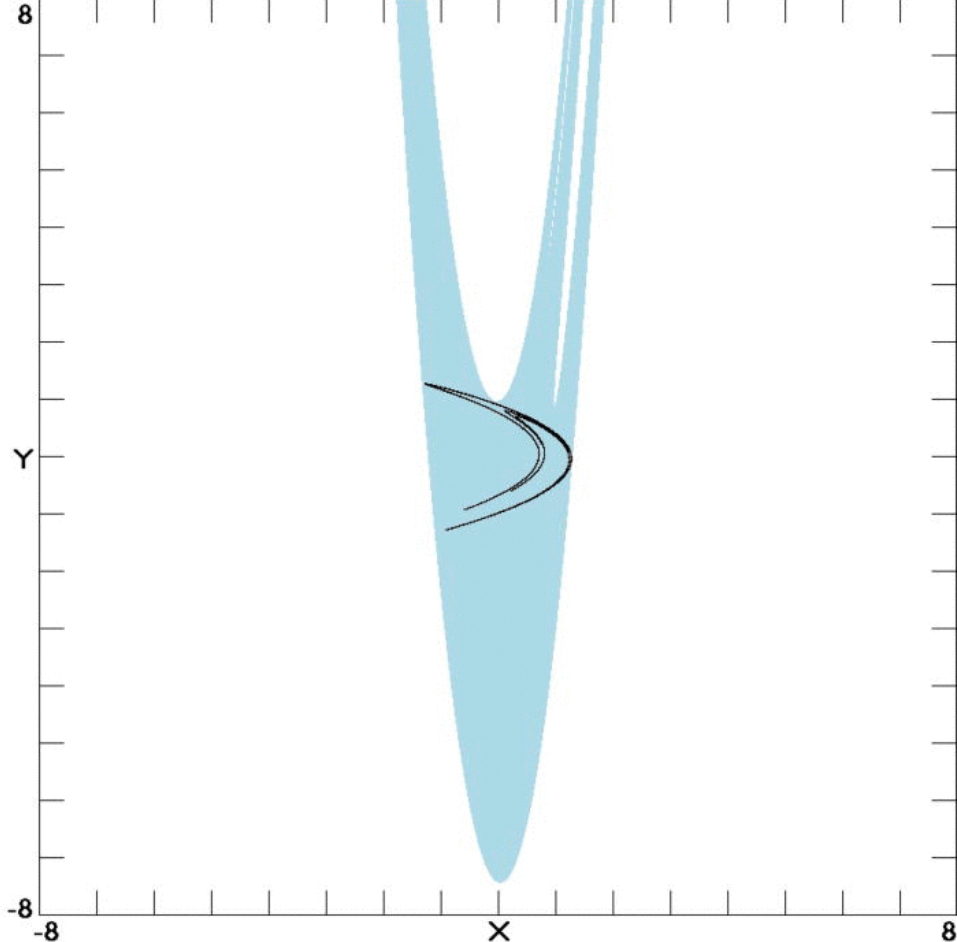
\includegraphics[width=.4\linewidth]{figures/IMG_0769.jpg} \\
        \small (a)
    \end{tabular} \qquad
    \begin{tabular}[b]{c}
        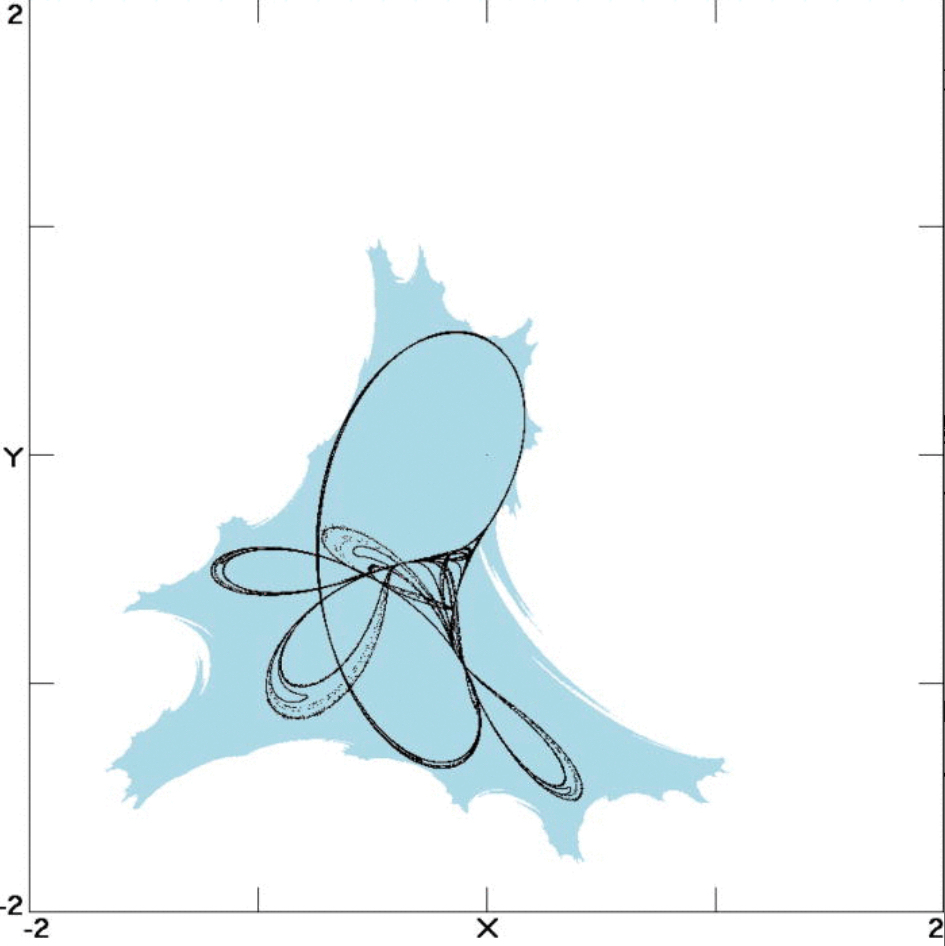
\includegraphics[width=.4\linewidth]{figures/IMG_0770.jpg} \\
        \small (b)
    \end{tabular}



    \caption[Examples of Basin Classes]{Examples of basin classes. The black lines represent the attractors and the blue areas the basins of attraction. Note that in (a) parts of the basin extend to infinity while (b) is bounded. \cite{classify}}%
    \label{fig:classes}%
\end{figure}

Knowing that BoA are not uniform in most cases, the direction of a disturbance within the phase space matters. If the basin border is particularly close to the attractor at any point, the system will be less robust to disturbances in that direction. Comparable to the methodology in Section~\ref{Residual Force Polytopes} Horibe et al.\ \cite{quant} have considering the worst case scenario by finding the shortest distance from the attractor to the boundary of the BoA.
This minimal radius of the BoA is a more conservative measure of robustness. It also allows to disregard complicated parts of the basin that extend to infinity or have strong fractal properties. In \cite{integr} this robustness measure was also determined, however under the name "Integrity Measure".
Coinciding with the goals of this project, \cite{quant} have used this robustness formulation to successfully optimize the physical design of inverted multi link pendulums with respect to control effort.
 
\subsection{Numerical Methods for Basin of Attraction Analysis} \label{Numerical Methods}
In order to quantify the robustness of a system using the BoA, the shape of the basin needs to be explored. Solving the systems of differential equations analytically is often not feasible, requiring numerical methods to be applied. The general procedure is first the sampling of a finite set of initial conditions from the continuous phase space and then integration of the differential equations. One popular method, applied by Brzeski et al.\ \cite{multistable} to quantify the responses of multistable systems, uses Monte Carlo methods for the sampling in which the initial conditions are chosen randomly from a given probability distribution. Finding the corresponding trajectories and determining whether they converge to the attractor gives a picture of the basin geometry. \cite{limitsBoA} explores potential issues with this method and finds that chaotic systems can lead to large cumulative errors in the integration of the trajectories. Furthermore the fraction of space that the basins take up tends to become smaller in higher dimensions, leading to more samples having to be evaluated and in turn increasing the computational cost.
An alternative approach are the “Cell Mapping Methods”, first summarized in \cite{cell1} and recently updated in \cite{cell2} as a comprehensive book. For cell mapping methods, the entire phase space is discretized along each dimension, resulting in a grid of possibly high dimensional, equally sized cells. The center point of each cell is chosen as the initial condition with which the differential equations are solved. The resulting trajectory is computed for a short time period to determine the mapping to a following cell. Repeating this procedure for all cells reveals the global behavior of the system dynamics. The benefit here is that integration errors are only local and stay confined to the basin boundaries. In addition, as the integration of the differential equations is bound to short intervals, each evaluation becomes computationally cheaper.

\begin{figure}[h]
    
    \centering
    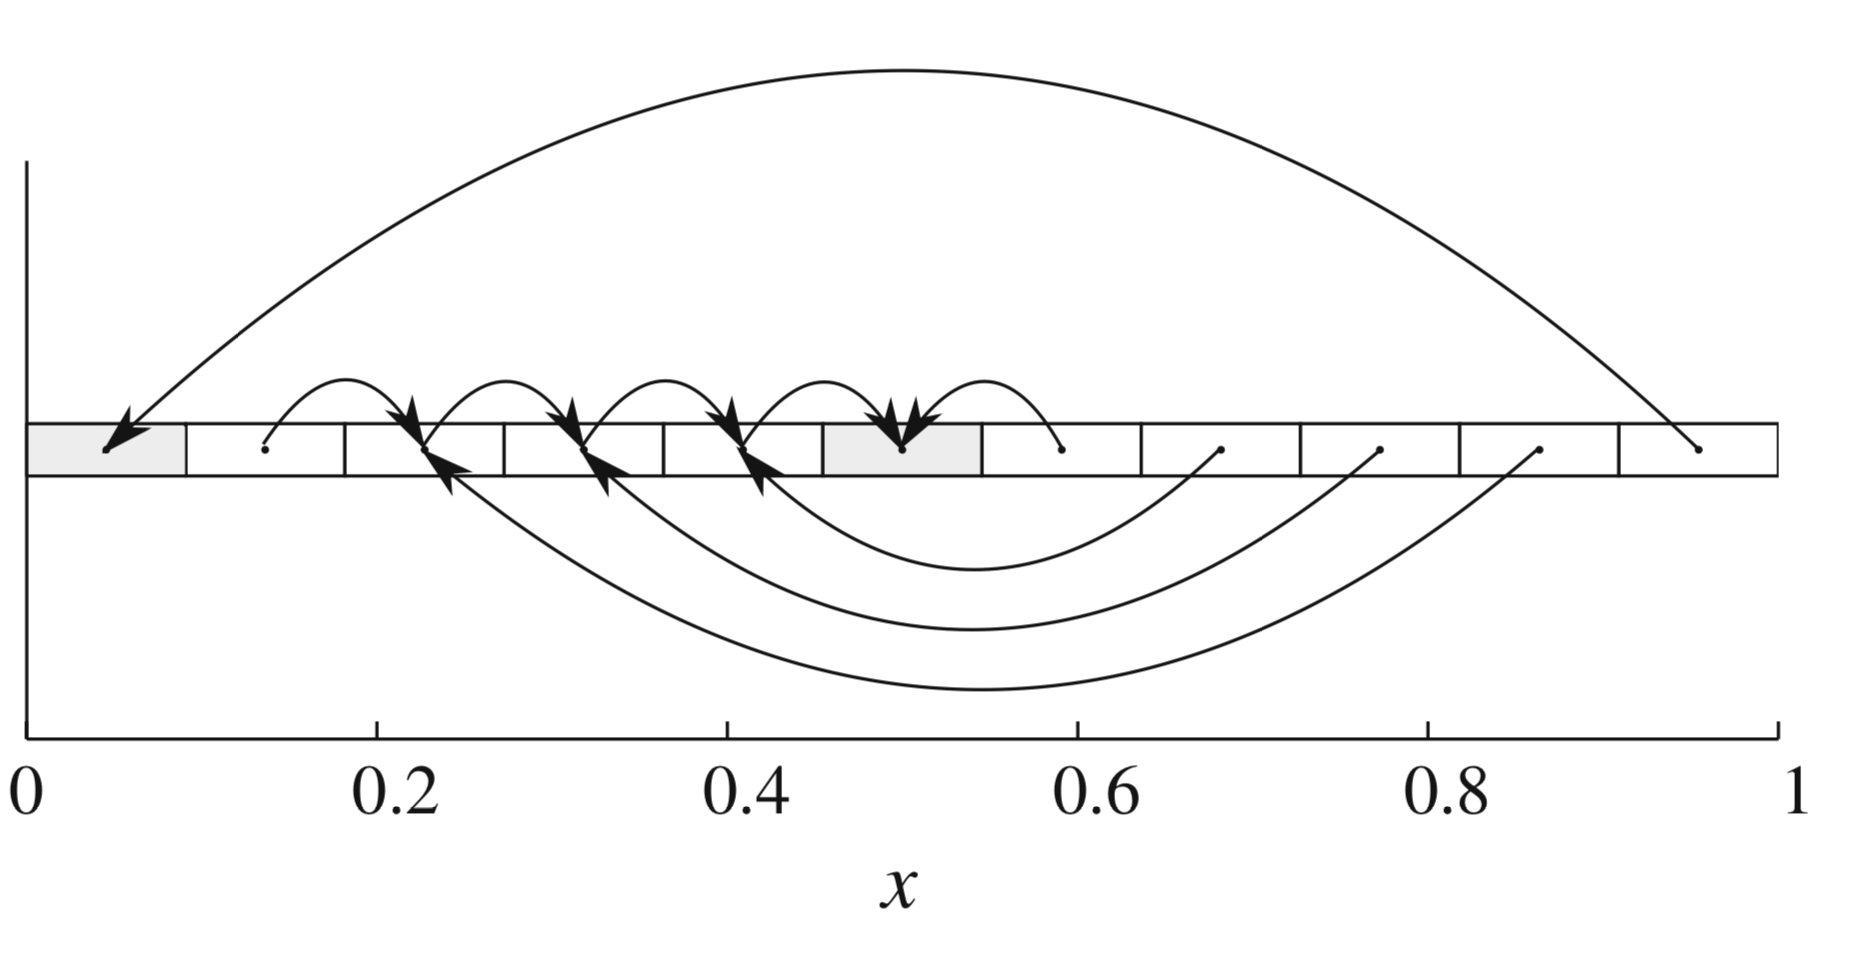
\includegraphics[width=.5\linewidth]{figures/1d-cm.jpg}
    \caption[One dimensional SCM]{One dimensional SCM. The rightmost cell goes to infinity, which is mapped to the 0 position, the so called sink-cell. With the remaining cells an attractor can be seen at x = 0.5. \cite{cell1}}
    \label{fig:1d-cm}
\end{figure}

This deterministic mapping between cells represents the Simple Cell Mapping (SCM). An issue with it is that it does not consider the infinite amount of initial conditions covered by each cell, which could all potentially result in vastly different trajectories. This discrepancy is overcome with the General Cell Mapping (GCM), a stochastic approach where from each starting cell the probability of landing in any other cell is found. This problem translates to a Markov chain representation, which has been well researched and for which efficient algorithms exist. The GCM is also better at dealing with fractal basin boundaries and can handle chaotic systems. As seen \cite{cell2}, there are many extensions to, as well as hybrids of the SCM and GCM methods, yielding better results. But of course cell mapping methods do have their limitations. 
As always, the curse of dimensionality persists and adding more dimensions exponentially increases the number of cells that have to be evaluated. For the overarching project systems with many degrees of freedom need to be analyzed, resulting in high dimensional phase spaces and increasing the computational cost. To overcome this hurdle, there have been efforts in parallelization of the computation by \cite{sixdim},\cite{parallel} and \cite{integr}, allowing for the exploration of higher dimensional systems, with promising results (see Figure~\ref{fig:sboa}). Given the results from any of the Cell Mapping Measures, either the volume or the minimal radius of a BoA can then be found to act as the concrete measure of robustness. 

\begin{figure}[ht]
    \centering
    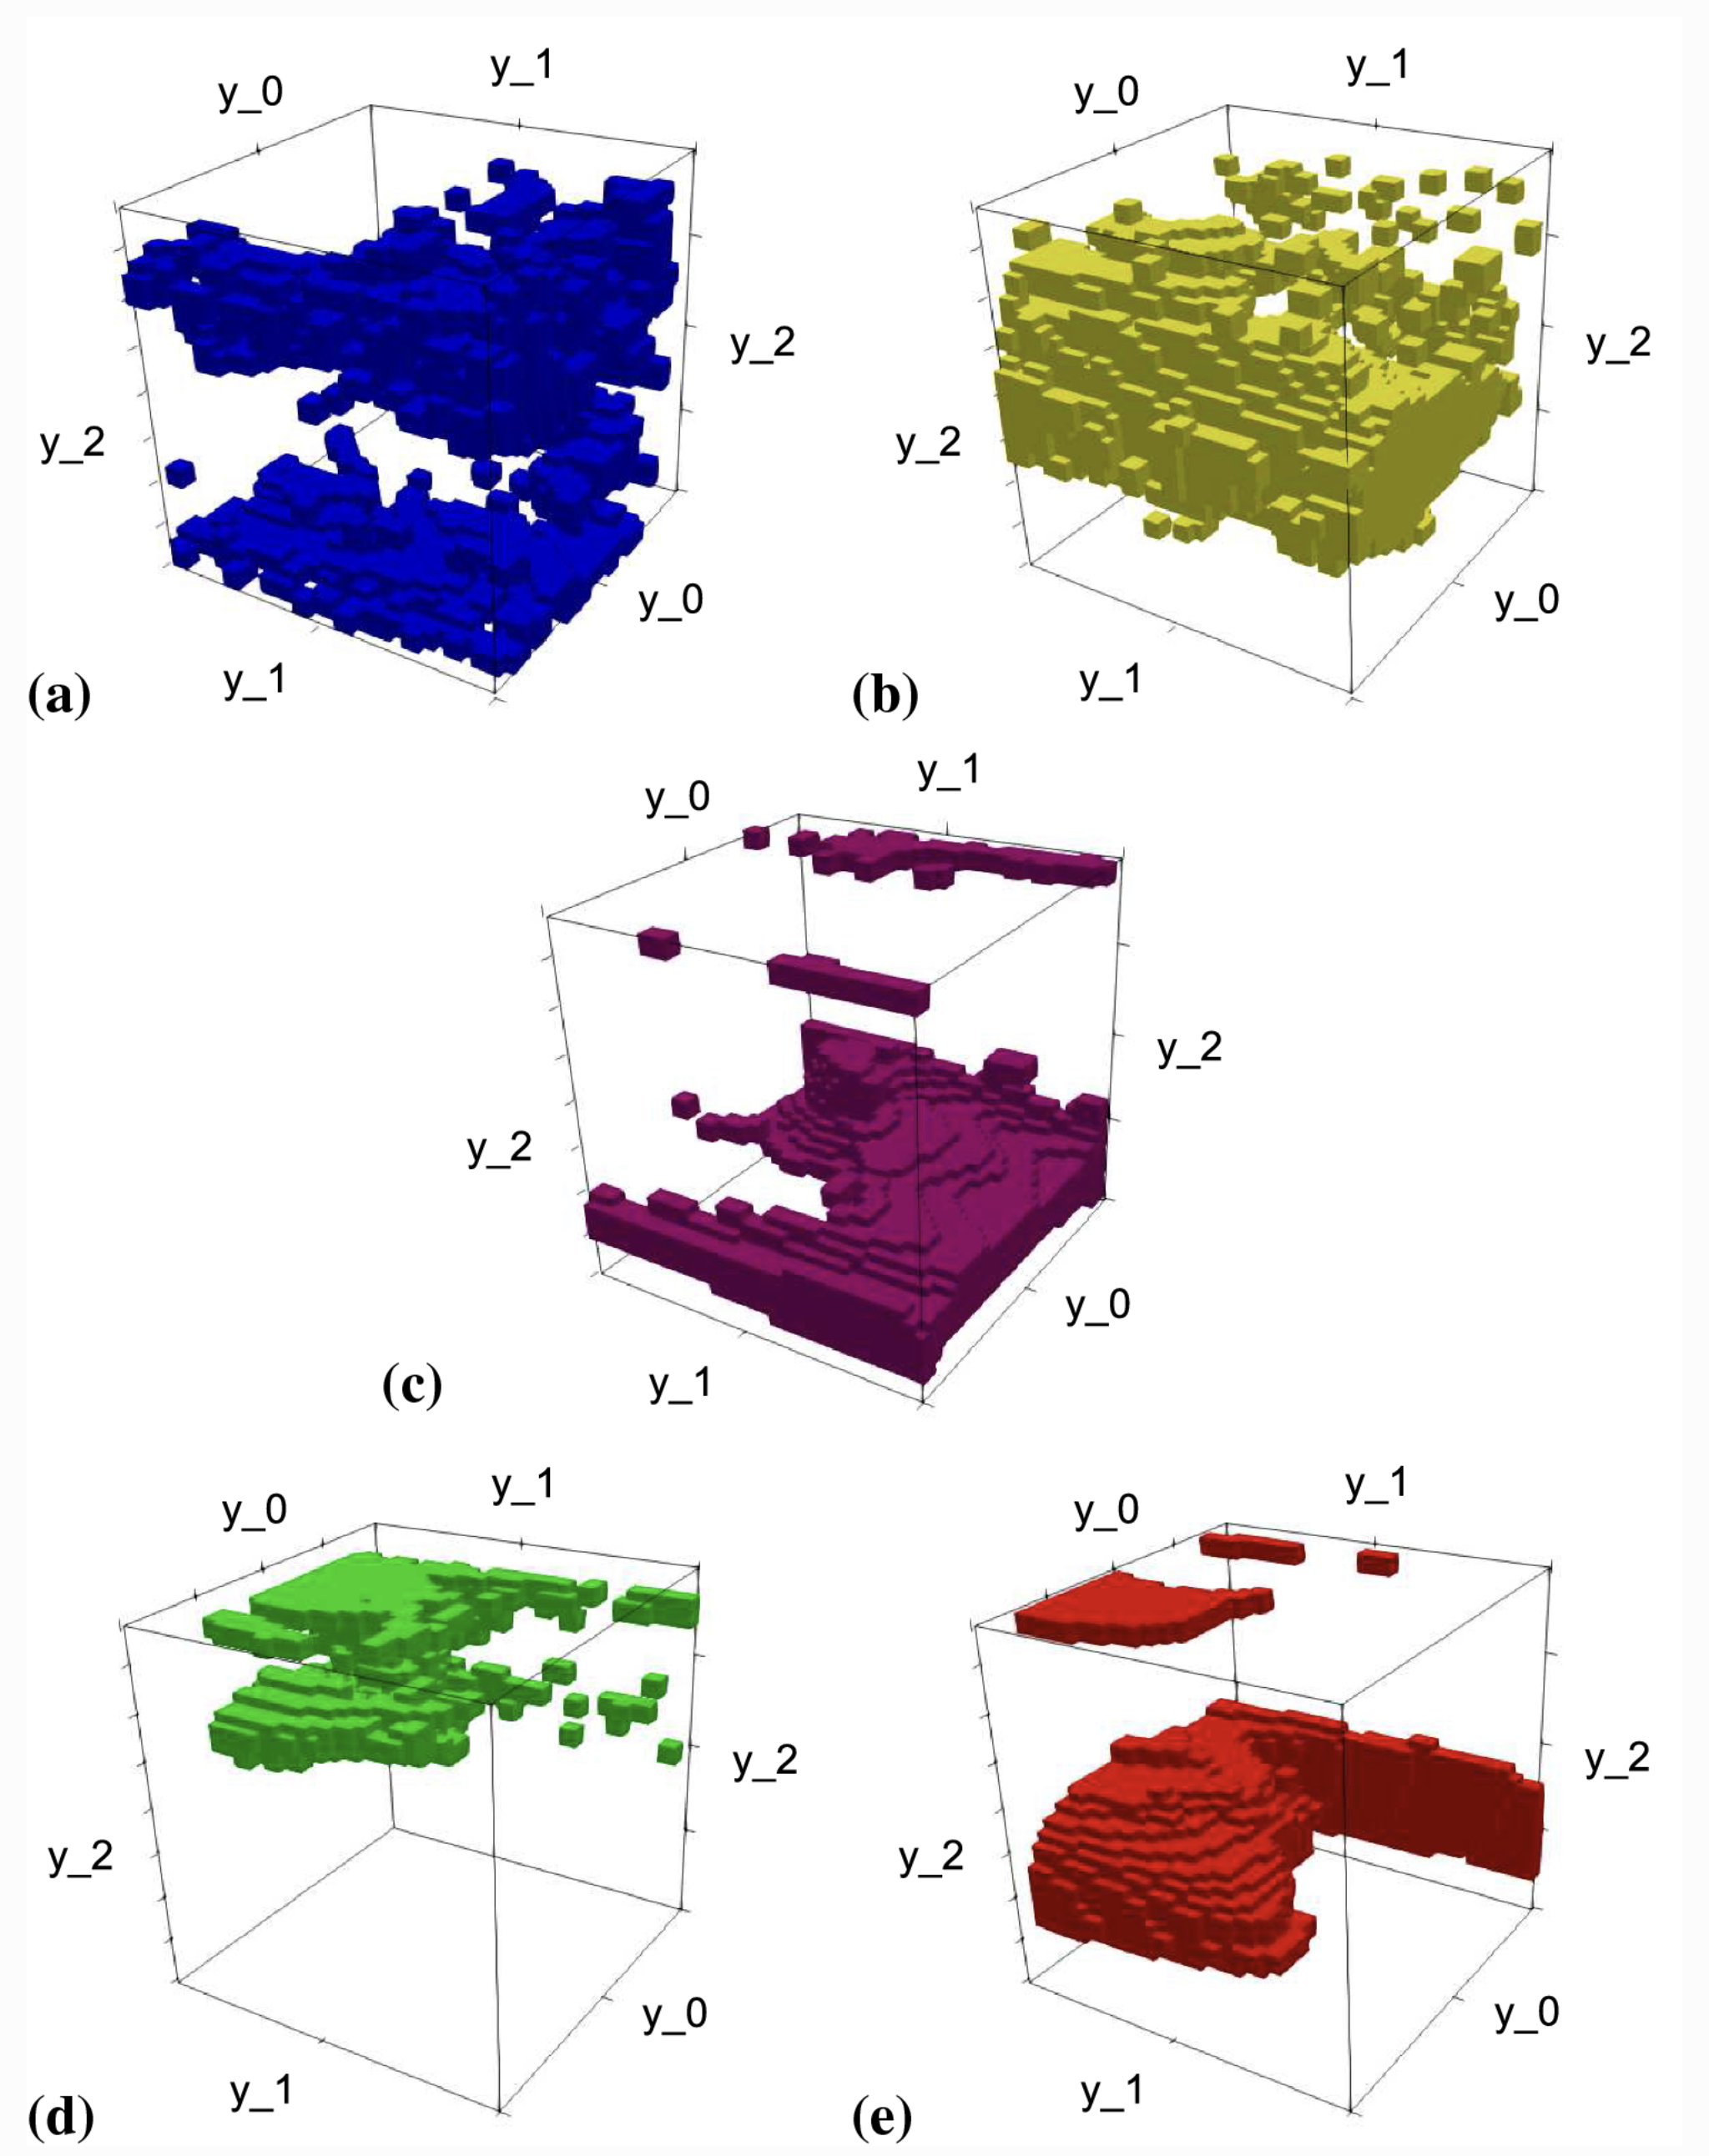
\includegraphics[width=.5\linewidth]{figures/IMG_0783.jpg}
    \caption[Six Dimensional Basin of Attraction]{3D sections of multiple six dimensional Basins of Attraction. \cite{sixdim}}
    \label{fig:sboa}
\end{figure}


\begin{figure}[h]
    \centering
    %\fontsize{7}{10}\selectfont
    %\includesvg[width=.9\linewidth]{bisection.svg}
    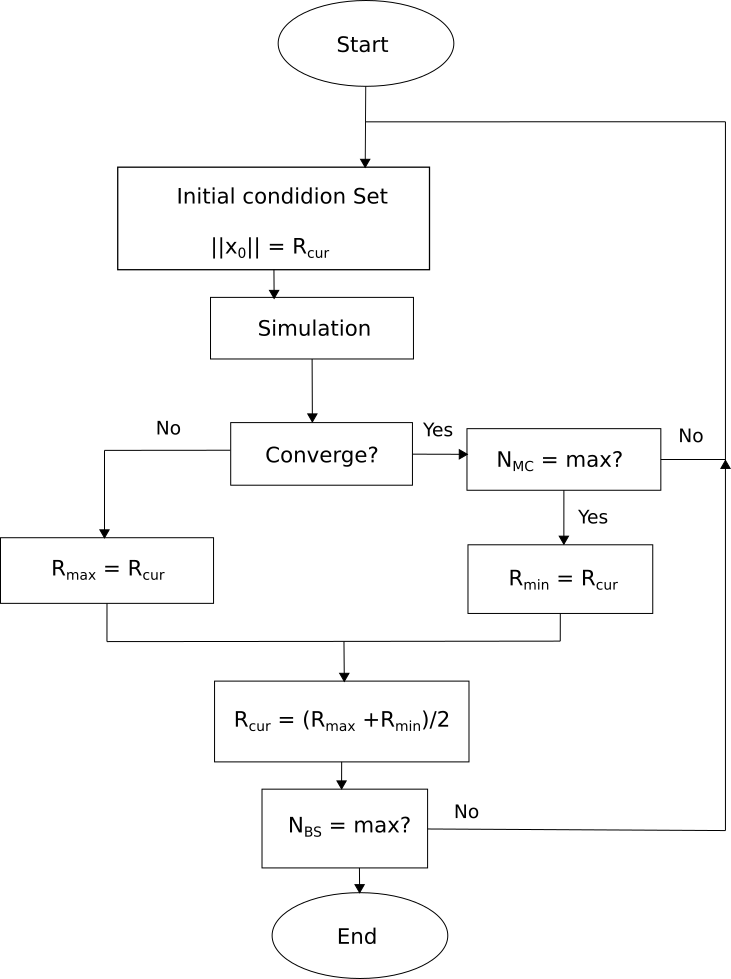
\includegraphics[width=.5\linewidth]{figures/bisection.png}
    \caption[Biseciton Algorithm]{Bisection Algorithm. Using two initial guesses $N_{MC}$ samples at the current radius are evaluated for convergence. If all samples converge the minimal radius is updated, otherwise the maximal radius. This is repeated for $N_{BS}$ iterations. \cite{quant}}
    \label{fig:alg}
\end{figure}

Looking again at \cite{quant}, robustness was determined without a global exploration, but by strategically sampling initial conditions and using the bisection algorithm to approximate the minimal radius, as seen in Figure~\ref{fig:alg}. For this method the trajectories had to again be evaluated until their convergence could be determined. Still, with the strong reduction of the total number of evaluations to be performed, the computational cost of quantifying the robustness was greatly decreased. 



\iffalse
\newpage
\section{Discussion} \label{Discussion}
The previous sections presented robustness definitions in different fields as well as concrete measures applicable to nonlinear systems. Cell Mapping Methods and random sampling in combination with trajectory evaluation were discussed and their shortcomings as well as their benefits were pointed out. While Cell Mapping Methods have low evaluation costs for each of their cells, the total computational cost rises exponentially when applied to higher dimensions. At the same time they are easily parallelizable, leaving a possibility of reducing the total computational time. The random sampling methods face similar issues in high dimensions with shrinking basin ratios and large errors in the trajectory exploration caused by chaos. Given the geometry of the BoA, the volume of the basin and its minimal radius were presented as specific measures for robustness. The later introduced bisection method presented an improvement on the random sampling approach by determining only the minimal radius of the BoA. An important assumption for this method is the knowledge of the location of the BoA, as the algorithm depends on knowing the distance from the center of attraction. 
The bisection method seems to be the most promising, especially as it has been applied to a problem very similar to the goal of the project. This however also assumes that the input data is a set of differential equations. Given experimental data, it might make sense to incorporate them into the Cell Mapping Methods, possibly mitigating the need for computing the trajectories. In any case, these are all very powerful tools, which can obtain excellent results, given a certain amount of computational resources.
\fi